\section{积与 Segre 映射}\label{sec:products-and-segre-maps}

本节的首要目标是研究射影簇的积. 射影情形下积的概念要比仿射情形复杂不少. 复杂性来自这样一个事实: 在仿射情形有自然等同 $\mathbb{A}^{m}\times\mathbb{A}^{n}=\mathbb{A}^{m+n}$, 但 $\mathbb{P}^{m}\times\mathbb{P}^{n}$ 与 $\mathbb{P}^{m+n}$ 之间没有这样的等同, 建议读者思考其中的原因. 事实上, 起初甚至并不清楚怎样把 $\mathbb{P}^{m}\times\mathbb{P}^{n}$ 本身解释为射影簇. 第一项任务是把 $\mathbb{P}^{m}\times\mathbb{P}^{n}$ 单射到一个更大的射影空间中, 从而将其解释为射影簇. 为此使用 Segre 映射, 它们以意大利数学家 Corrado Segre (1863--1924) 命名.

\begin{Definition}{Segre 映射}\leavevmode\label{def:segre-map}
对任意 $m,n\ge0$, 从 $\mathbb{P}^{m}\times\mathbb{P}^{n}$ 到 $\mathbb{P}^{(m+1)(n+1)-1}$ 的 \emph{Segre 映射} $S_{m,n}$ 由下式给出:
\[
  S_{m,n}=[x_{0}y_{0}:x_{0}y_{1}:\cdots:x_{m}y_{n-1}:x_{m}y_{n}],
\]
其中定义中的单项式是所有可能的乘积 $x_{i}y_{j}$.
\end{Definition}

为了理解这个定义, 我们先看第一个有意思的例子.

\begin{Example}{Segre 映射 $S_{1,1}$}\leavevmode\label{ex:segre-product-of-two-projective-lines}
考察 $m=n=1$ 时的 Segre 映射:
\[
  \begin{aligned}
    S_{1,1}:\mathbb{P}^{1}\times\mathbb{P}^{1}&\to\mathbb{P}^{3}\\
    ([a_{0}:a_{1}],[b_{0}:b_{1}])&\mapsto[a_{0}b_{0}:a_{0}b_{1}:a_{1}b_{0}:a_{1}b_{1}].
  \end{aligned}
\]
注意, 缩放任一个 $\mathbb{P}^{1}$ 中的齐次坐标只会使像中的所有坐标作相同的缩放. 此外, 可以验证
\[
  a_{0}b_{0}=a_{0}b_{1}=a_{1}b_{0}=a_{1}b_{1}=0
  \implies a_{0}=a_{1}=0\quad\text{或}\quad b_{0}=b_{1}=0.
\]
这两个观察合起来意味着, $S_{1,1}$ 在 $\mathbb{P}^{1}\times\mathbb{P}^{1}$ 的每一点均为良定义. 建议读者推广这一点, 验证 $S_{m,n}$ 在 $\mathbb{P}^{m}\times\mathbb{P}^{n}$ 的每一点均为良定义 (Exercise~\ref{ex:segre-map-well-defined}).
\end{Example}

尽管 Segre 映射在定义域的每一点均为良定义, 此时问它们是不是正则映射还没有意义, 原因只在于尚未赋予定义域射影簇结构. 事实上, 我们恰要利用 Segre 映射, 赋予 $\mathbb{P}^{m}\times\mathbb{P}^{n}$ 在 $\mathbb{P}^{(m+1)(n+1)-1}$ 中的射影簇结构. 为此, 引入一种能方便地组织 $\mathbb{P}^{(m+1)(n+1)-1}$ 的坐标的记号.

注意 $\mathbb{P}^{(m+1)(n+1)-1}$ 有 $(m+1)(n+1)$ 个齐次坐标; 将这些坐标记为 $z_{ij}$, 其中 $0\le i\le m$ 且 $0\le j\le n$. 方便的是, 可以自然地把这些坐标排成一个 $m\times n$ 矩阵 $A(z)$, 其第 $ij$ 项为 $z_{ij}$. 按这样的标记, 约定 Segre 映射 $S_{m,n}$ 的 $z_{ij}$ 坐标为 $x_{i}y_{j}$. 现在用这个记号描述 Segre 映射的像.

\begin{Proposition}{Segre 映射单射到一个射影簇上}\leavevmode\label{prop:segre-map-injective-with-determinantal-image}
对任意 $m,n\ge0$, Segre 映射 $S_{m,n}$ 是 $\mathbb{P}^{m}\times\mathbb{P}^{n}$ 到射影簇 $Z_{m,n}\subseteq\mathbb{P}^{(m+1)(n+1)-1}$ 上的单射, 其中
\[
  Z_{m,n}=\mathcal{V}\bigl(\{z_{ij}z_{k\ell}-z_{i\ell}z_{kj}
      \mid 0\le i,k\le m,\ 0\le j,\ell\le n\}\bigr).
\]
\end{Proposition}
\begin{Proof}
\BookPairedNote{
我们证明 $S_{m,n}$ 的像等于 $Z_{m,n}$, 而把 $S_{m,n}$ 是单射的验证留作习题 (Exercise~\ref{ex:segre-map-injective}).
}{
$Z_{m,n}$ 由矩阵 $A(z)$ 的所有 $2\times2$ 子式定义, 因此是\textquotedbl{}行列式簇\textquotedbl{}的一个例子.
}
为证明 $S_{m,n}$ 的像包含在 $Z_{m,n}$ 中, 只须证明 $z_{ij}z_{k\ell}-z_{i\ell}z_{kj}$ 在 $S_{m,n}$ 像中的任一点消没. 这来自对任意 $(a,b)\in\mathbb{P}^{m}\times\mathbb{P}^{n}$, 都有
\[
  (a_{i}b_{j})(a_{k}b_{\ell})-(a_{i}b_{\ell})(a_{k}b_{j})=0.
\]
反过来, 为证明 $Z_{m,n}$ 包含在 $S_{m,n}$ 的像中, 令 $c\in Z_{m,n}$. 这意味着 $A(c)$ 的所有 $2\times2$ 子式都消没, 从而 $A(c)$ 的秩至多为一; 换句话说, $A(c)$ 的每一行都是某一行的倍数. 由于必有至少一行非零, 不妨设首行非零, 并将其记为 $b=(b_{0},\ldots,b_{n})$. 令 $a_{i}\in K$ 为使 $A(c)$ 的第 $i$ 行等于 $a_{i}b$ 的值. 容易验证
\[
  c=S_{m,n}([1:a_{1}:\cdots:a_{m}],[b_{0}:b_{1}:\cdots:b_{n}]),
\]
所以 $c$ 在 $S_{m,n}$ 的像中.
\end{Proof}

\begin{Example}{$S_{1,1}$ 的像}\leavevmode\label{ex:segre-image-of-two-projective-lines}
再考察 $m=n=1$ 的情形, 把 $\mathbb{P}^{3}$ 的坐标记为 $z_{00},z_{01},z_{10},z_{11}$. Proposition~\ref{prop:segre-map-injective-with-determinantal-image} 表明, $S_{1,1}$ 是到 $\mathbb{P}^{3}$ 中由以下 $2\times2$ 行列式的消没定义的射影簇上的单射:
\[
  \det\begin{pmatrix}
    z_{00}&z_{01}\\
    z_{10}&z_{11}
  \end{pmatrix}=z_{00}z_{11}-z_{01}z_{10}.
\]
\end{Example}

Proposition~\ref{prop:segre-map-injective-with-determinantal-image} 的重要性在于, 它将积 $\mathbb{P}^{m}\times\mathbb{P}^{n}$ 与 $\mathbb{P}^{(m+1)(n+1)-1}$ 中的一个射影簇等同, 从而给出了将积本身视为射影簇的一种自然方式. 下一个结果表明, 可以用 Segre 映射自然地把任意两个射影簇的积视为射影簇, 不限于射影空间的积.

\begin{Proposition}{射影簇的积}\leavevmode\label{prop:segre-map-restricts-to-product-of-projective-varieties}
若 $X\subseteq\mathbb{P}^{m}$ 和 $Y\subseteq\mathbb{P}^{n}$ 为射影簇, 则 Segre 映射 $S_{m,n}$ 限制为从 $X\times Y$ 到 $\mathbb{P}^{(m+1)(n+1)-1}$ 中的一个射影簇上的单射.
\end{Proposition}
\begin{Proof}
设 $X=\mathcal{V}(\mathcal{S})$ 且 $Y=\mathcal{V}(\mathcal{T})$, 其中 $\mathcal{S}\subseteq K[x_{0},\ldots,x_{m}]$ 且 $\mathcal{T}\subseteq K[y_{0},\ldots,y_{n}]$. 对每个 $f\in\mathcal{S}$ 和 $g\in\mathcal{T}$, 以及每个 $0\le i\le n$ 和 $0\le j\le m$, 定义
\[
  f_{i}=f(z_{0i},z_{1i},\ldots,z_{mi})
  \qquad\text{和}\qquad
  g_{j}=g(z_{j0},z_{j1},\ldots,z_{jn}).
\]
令 $\mathcal{S}'$ 为所有这类 $f_{i}$ 的集合, $\mathcal{T}'$ 为所有这类 $g_{j}$ 的集合. 建议读者验证 (Exercise~\ref{ex:equations-for-segre-image-of-product})
\[
  S_{m,n}(X\times Y)=S_{m,n}(\mathbb{P}^{m}\times\mathbb{P}^{n})
  \cap\mathcal{V}(\mathcal{S}'\cup\mathcal{T}').
\]
由 Proposition~\ref{prop:segre-map-injective-with-determinantal-image} 可知, $S_{m,n}$ 是单射, 且 $S_{m,n}(\mathbb{P}^{m}\times\mathbb{P}^{n})$ 是射影簇. 由于射影簇的交本身也是射影簇, 我们得出 $S_{m,n}(X\times Y)$ 是射影簇.
\end{Proof}

现在用 Segre 映射把 $X\times Y$ 与射影簇 $S_{m,n}(X\times Y)$ 等同, 从而在射影簇的范畴内定义积.

\begin{Definition}{射影簇的积}\leavevmode\label{def:product-of-projective-varieties}
若 $X\subseteq\mathbb{P}^{m}$ 和 $Y\subseteq\mathbb{P}^{n}$ 为射影簇, 则它们的\emph{积} $X\times Y$ (作为射影簇) 定义为射影簇
\[
  S_{m,n}(X\times Y)\subseteq\mathbb{P}^{(m+1)(n+1)-1}.
\]
\end{Definition}

\begin{Example}{一张双直纹曲面}\leavevmode\label{ex:segre-quadric-is-doubly-ruled}
我们停下来直观地看一下射影簇 $\mathbb{P}^{1}\times\mathbb{P}^{1}$. 由 Definition~\ref{def:product-of-projective-varieties} 和 Example~\ref{ex:segre-image-of-two-projective-lines}, 它等于射影簇 $\mathcal{V}(z_{00}z_{11}-z_{01}z_{10})\subseteq\mathbb{P}^{3}$.

\BookPairedFigure{
考察 $z_{00}\ne0$ 的仿射限制, 它是仿射曲面
\[
  \mathcal{V}_{\mathbb{A}}(z_{11}-z_{01}z_{10})\subseteq\mathbb{A}^{3}.
\]
右图描绘的是这一仿射限制在 $\mathbb{R}$ 上的情形. 可以看出这张曲面是双直纹的: 有两种不同的方式将它看作直线的不交并.
}{
\phantomsection\label{fig:segre-doubly-ruled-surface}%
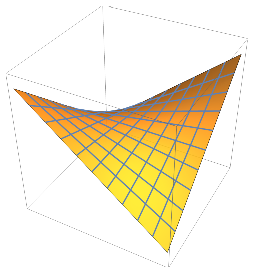
\includegraphics[width=\linewidth]{figures/segre-doubly-ruled-surface.pdf}
}
这一仿射限制的双直纹反映了一个更一般的事实: 射影曲面 $\mathbb{P}^{1}\times\mathbb{P}^{1}\subseteq\mathbb{P}^{3}$ 也是双直纹的, 有两种不同的方式将它实现为 $\mathbb{P}^{3}$ 中 (射影) 直线的不交并. $\mathbb{P}^{1}\times\mathbb{P}^{1}$ 的两族直纹由 $\mathbb{P}^{3}$ 中形如
\[
  \{a\}\times\mathbb{P}^{1}\qquad\text{和}\qquad\mathbb{P}^{1}\times\{b\}
\]
的子集给出, 建议读者在 Exercise~\ref{ex:two-rulings-of-segre-quadric} 中探究这一点.
\end{Example}

把积 $X\times Y$ 实现为射影簇后, 就可以讨论从 $X\times Y$ 出发和到 $X\times Y$ 的正则映射. 下面的结果涉及从积出发的正则映射中最重要的两个例子: 两个投影映射.

\begin{Proposition}{投影映射是正则的}\leavevmode\label{prop:product-projections-are-regular}
若 $X\subseteq\mathbb{P}^{m}$ 和 $Y\subseteq\mathbb{P}^{n}$ 为射影簇, 则投影映射 $\pi_{1}:X\times Y\to X$ 和 $\pi_{2}:X\times Y\to Y$ 都是正则的.
\end{Proposition}
\begin{Proof}
只考虑 $\pi_{1}$; $\pi_{2}$ 的论证可由对称性得到. 只需注意, 对任意 $c=(a,b)\in X\times Y\subseteq\mathbb{P}^{(m+1)(n+1)-1}$, 可以用如下分片表达式写出 $\pi_{1}(c)$:
\[
  \pi_{1}(c)=\begin{cases}
    [c_{00}:c_{10}:\cdots:c_{m0}] & c\notin\mathcal{V}(z_{00},z_{10},\ldots,z_{m0})\\
    \vdots & \vdots\\
    [c_{0n}:c_{1n}:\cdots:c_{mn}] & c\notin\mathcal{V}(z_{0n},z_{1n},\ldots,z_{mn}).
  \end{cases}
\]
为验证上述 $\pi_{1}$ 的表达式, 设 $c=(a,b)\in X\times Y$. 则 $c$ 的 $z_{ij}$ 坐标为 $a_{i}b_{j}$. 注意, $a$ 至少有一个非零坐标, $b$ 也至少有一个非零坐标. 若 $b_{j}\ne0$, 则 $c\notin\mathcal{V}(z_{0j},z_{1j},\ldots,z_{mj})$, 并且计算得
\[
  \begin{aligned}
    [c_{0j}:c_{1j}:\cdots:c_{mj}]
      &=[a_{0}b_{j}:a_{1}b_{j}:\cdots:a_{m}b_{j}]\\
      &=[a_{0}:a_{1}:\cdots:a_{m}]=\pi_{1}(c),
  \end{aligned}
\]
验证了上述 $\pi_{1}(c)$ 的表达式.
\end{Proof}

正如可以取射影簇的积, 也可以取映到各因子的映射的积. 下一个结果涉及正则映射的积.

\begin{Proposition}{正则映射的积是正则的}\leavevmode\label{prop:products-of-projective-regular-maps-are-regular}
令 $W\subseteq\mathbb{P}^{\ell}$, $X\subseteq\mathbb{P}^{m}$, $Y\subseteq\mathbb{P}^{n}$ 为射影簇. 若 $F:W\to X$ 和 $G:W\to Y$ 都是正则映射, 则函数
\[
  \begin{aligned}
    F\times G:W&\to X\times Y\\
    a&\mapsto(F(a),G(a))
  \end{aligned}
\]
是正则映射.
\end{Proposition}
\begin{Proof}
令 $p\in W$. 由正则映射的定义, 存在齐次多项式
\[
  f_{0},\ldots,f_{m},g_{0},\ldots,g_{n}\in K[w_{0},\ldots,w_{\ell}],
\]
使 $p\notin\mathcal{V}(f_{0},\ldots,f_{m})\cup\mathcal{V}(g_{0},\ldots,g_{n})$, 且
\[
  F(a)=[f_{0}(a):\cdots:f_{m}(a)]
  \qquad\text{对所有 }a\in W\setminus\mathcal{V}(f_{0},\ldots,f_{m}),
\]
以及
\[
  G(a)=[g_{0}(a):\cdots:g_{n}(a)]
  \qquad\text{对所有 }a\in W\setminus\mathcal{V}(g_{0},\ldots,g_{n}).
\]
由此可知 $p\notin\mathcal{V}(\{f_{i}g_{j}\mid0\le i\le m,\ 0\le j\le n\})$. 由射影簇积的定义, 对所有 $a\in W\setminus\mathcal{V}(\{f_{i}g_{j}\mid0\le i\le m,\ 0\le j\le n\})$, 有
\[
  \begin{aligned}
  (F\times G)(a)
  &=[f_{0}(a)g_{0}(a):f_{0}(a)g_{1}(a):\cdots:\\
  &\hspace{7em}f_{m}(a)g_{n-1}(a):f_{m}(a)g_{n}(a)].
  \end{aligned}
\]
因此 $F\times G$ 可以局部用多项式 $f_{i}g_{j}$ 描述, 这验证了 $F\times G$ 是正则的.
\end{Proof}

前述结果的一个重要推论如下, 它说明积的内在性质只取决于各因子的内在性质.

\begin{Corollary}{积保持同构}\leavevmode\label{cor:products-preserve-projective-isomorphisms}
令 $X,X',Y,Y'$ 为射影簇. 若 $X\cong X'$ 且 $Y\cong Y'$, 则
\[
  X\times Y\cong X'\times Y'.
\]
\end{Corollary}
\begin{Proof}
令 $F:X\to X'$ 和 $G:Y\to Y'$ 为同构. 由于投影映射正则, 将 $F$ 和 $G$ 分别与相应的投影映射复合 (先作用投影), 可得到正则映射
\[
  F\circ\pi_{1}:X\times Y\to X'
  \qquad\text{和}\qquad
  G\circ\pi_{2}:X\times Y\to Y'.
\]
这两个正则映射的积于是为正则映射
\[
  \begin{aligned}
    X\times Y&\to X'\times Y'\\
    (a,b)&\mapsto(F(a),G(b)).
  \end{aligned}
\]
由于 $F$ 和 $G$ 都是同构, 它们有正则逆映射. 对 $F^{-1}$ 和 $G^{-1}$ 重复上述过程, 得到正则映射
\[
  \begin{aligned}
    X'\times Y'&\to X\times Y\\
    (a,b)&\mapsto(F^{-1}(a),G^{-1}(b)).
  \end{aligned}
\]
$X\times Y$ 和 $X'\times Y'$ 之间上述一对正则映射互逆, 由此得出 $X\times Y\cong X'\times Y'$.
\end{Proof}

若 $X\subseteq\mathbb{P}^{m}$ 和 $Y\subseteq\mathbb{P}^{n}$ 为射影簇, 则我们已经证明, 它们的积 $X\times Y$ 是 $\mathbb{P}^{m}\times\mathbb{P}^{n}\subseteq\mathbb{P}^{(m+1)(n+1)-1}$ 中的射影簇. 自然要问: $\mathbb{P}^{m}\times\mathbb{P}^{n}$ 中还有其他射影簇吗? 确实有, 本节的最后一项任务就是用一种新的消没概念, 将它们刻画为消没集. 给定多项式 $f\in K[x_{0},\ldots,x_{m},y_{0},\ldots,y_{n}]$, 若 $f$ 在 $(a,b)$ 的任一代表元处取值均为零, 则称 $f$ 在点 $(a,b)\in\mathbb{P}^{m}\times\mathbb{P}^{n}$ 处消没. 于是以自然方式定义射影空间积上的消没算子 $\mathcal{V}=\mathcal{V}_{\mathbb{P}^{m}\times\mathbb{P}^{n}}$. 利用这个新的消没概念, 下面的结果给出 $\mathbb{P}^{m}\times\mathbb{P}^{n}$ 中所有射影簇的刻画, 无须显式提及 Segre 映射.

\begin{Proposition}{$\mathbb{P}^{m}\times\mathbb{P}^{n}$ 中的射影簇}\leavevmode\label{prop:projective-subvarieties-of-product-are-vanishing-sets}
令 $Z$ 为 $\mathbb{P}^{m}\times\mathbb{P}^{n}$ 的一个子集. 通过 Segre 映射将 $\mathbb{P}^{m}\times\mathbb{P}^{n}$ 视为射影簇后, $Z$ 本身是射影簇, 当且仅当对某个 $\mathcal{S}\subseteq K[x_{0},\ldots,x_{m},y_{0},\ldots,y_{n}]$, $Z$ 是消没集 $\mathcal{V}(\mathcal{S})\subseteq\mathbb{P}^{m}\times\mathbb{P}^{n}$.
\end{Proposition}

在证明之前来看一个例子.

\begin{Example}{$\mathbb{P}^{1}\times\mathbb{P}^{1}$ 中的对角线}\leavevmode\label{ex:diagonal-in-product-of-projective-lines}
由于 $\mathbb{P}^{1}$ 中的每个射影簇都是整个 $\mathbb{P}^{1}$ 或有限点集, $\mathbb{P}^{1}\times\mathbb{P}^{1}$ 中每个射影簇的积都具有下列四种形式之一: (i) $\mathbb{P}^{1}\times\mathbb{P}^{1}$; (ii) $\{a_{1},\ldots,a_{k}\}\times\mathbb{P}^{1}$, 其中 $\{a_{1},\ldots,a_{k}\}\subseteq\mathbb{P}^{1}$ 是某个 (可能为空的) 有限集; (iii) $\mathbb{P}^{1}\times\{b_{1},\ldots,b_{\ell}\}$, 其中 $\{b_{1},\ldots,b_{\ell}\}\subseteq\mathbb{P}^{1}$ 是某个 (可能为空的) 有限集; (iv) $\{a_{1},\ldots,a_{k}\}\times\{b_{1},\ldots,b_{\ell}\}$. Proposition~\ref{prop:projective-subvarieties-of-product-are-vanishing-sets} 使我们可以得到 $\mathbb{P}^{1}\times\mathbb{P}^{1}$ 中丰富得多的一类射影簇. 例如, 对角线
\[
  Z=\{(a,a)\mid a\in\mathbb{P}^{1}\}
\]
不属于上述四种类型, 但它是 $\mathbb{P}^{1}\times\mathbb{P}^{1}$ 中的一个射影簇. 为验证这一点, 回顾 $a_{0}b_{1}=a_{1}b_{0}$ 当且仅当 $[a_{0}:a_{1}]=[b_{0}:b_{1}]$, 所以
\[
  Z=\mathcal{V}(x_{0}y_{1}-x_{1}y_{0})\subseteq\mathbb{P}^{1}\times\mathbb{P}^{1}.
\]
因此, Proposition~\ref{prop:projective-subvarieties-of-product-are-vanishing-sets} 保证 $Z$ 是 $\mathbb{P}^{1}\times\mathbb{P}^{1}$ 中的射影簇.
\end{Example}

注意, 用与单个射影空间情形相似的论证, $\mathbb{P}^{m}\times\mathbb{P}^{n}$ 中任意消没集可写成
\[
  \mathcal{V}(f_{1},\ldots,f_{k}),
\]
其中 $f_{1},\ldots,f_{k}$ 都是\emph{双齐次的}, 即它们分别关于每一组变量齐次. 更进一步, 可以取每个 $f_{i}$ 关于两组变量的齐次次数相同. 这些断言的验证留作习题 (Exercise~\ref{ex:bihomogeneous-polynomials-define-vanishing-sets}); 在下面的证明中将用到它们.

\begingroup
\renewcommand{\AJProofBegin}{%
  \par\addvspace{\topsep}\noindent
  {\sffamily\bfseries\CJKfamily{pffont}Proof of Proposition~\ref{prop:projective-subvarieties-of-product-are-vanishing-sets}}\enspace\ignorespaces
}
\begin{Proof}
设 $Z\subseteq\mathbb{P}^{m}\times\mathbb{P}^{n}\subseteq\mathbb{P}^{(m+1)(n+1)-1}$ 为射影簇. 按定义, 这意味着
\[
  Z=\mathcal{V}(g_{1},\ldots,g_{\ell}),
\]
其中 $g_{1},\ldots,g_{\ell}\in K[z_{ij}\mid0\le i\le m,\ 0\le j\le n]$ 是次数分别为 $d_{1},\ldots,d_{\ell}$ 的齐次多项式. 在 Segre 映射下, 这对应于
\[
  Z=\{(a,b)\in\mathbb{P}^{m}\times\mathbb{P}^{n}
      \mid f_{k}(a,b)=0\text{ 对所有 }k=1,\ldots,\ell\},
\]
其中 $f_{k}(x,y)$ 是在 $g_{k}(z)$ 中对所有 $i,j$ 作代换 $z_{ij}=x_{i}y_{j}$ 得到的. 这就证明了命题的一个方向.

对另一方向, 设 $Z$ 为 $\mathbb{P}^{m}\times\mathbb{P}^{n}$ 中的消没集. 则 $Z=\mathcal{V}(f_{1},\ldots,f_{\ell})$, 其中
\[
  f_{1},\ldots,f_{\ell}\in K[x_{0},\ldots,x_{m},y_{0},\ldots,y_{n}].
\]
可以假设每个多项式都是双齐次的, 且关于两组变量的次数相同. 因此, 在 $f_{k}$ 的任何一个单项式中, $x$ 与 $y$ 因子的个数相同, 故可以把它们分成若干对, 构造多项式 $g_{k}\in K[z_{ij}]$, 使得作代换 $z_{ij}=x_{i}y_{j}$ 后 $g_{k}$ 变为 $f_{k}$. 因此 Segre 嵌入将 $Z$ 与 $(\mathbb{P}^{m}\times\mathbb{P}^{n})\cap\mathcal{V}(g_{1},\ldots,g_{\ell})$ 等同, 所以 $Z$ 是射影簇.
\end{Proof}
\endgroup

\BookExerciseHeading
\begin{BookExercises}
  \item\label{ex:segre-map-well-defined} 令 $a=[a_{0}:\cdots:a_{m}]\in\mathbb{P}^{m}$, $b=[b_{0}:\cdots:b_{n}]\in\mathbb{P}^{n}$.
  \begin{enumerate}
    \item 证明存在 $i,j$ 使 $a_{i}b_{j}\ne0$.
    \item 证明 $[a_{0}b_{0}:a_{0}b_{1}:\cdots:a_{m}b_{n-1}:a_{m}b_{n}]\in\mathbb{P}^{(m+1)(n+1)-1}$ 不依赖于 $a$ 或 $b$ 的齐次坐标的选取.
  \end{enumerate}
  \item\label{ex:segre-map-injective} 证明 Segre 映射 $S_{m,n}:\mathbb{P}^{m}\times\mathbb{P}^{n}\to\mathbb{P}^{(m+1)(n+1)-1}$ 是单射.
  \item\label{ex:equations-for-segre-image-of-product} 令 $X=\mathcal{V}(\mathcal{S})\subseteq\mathbb{P}^{m}$ 和 $Y=\mathcal{V}(\mathcal{T})\subseteq\mathbb{P}^{n}$, 其中 $\mathcal{S}\subseteq K[x_{0},\ldots,x_{m}]$ 且 $\mathcal{T}\subseteq K[y_{0},\ldots,y_{n}]$. 对每个 $f\in\mathcal{S}$ 和 $g\in\mathcal{T}$, 以及每个 $0\le i\le n$ 和 $0\le j\le m$, 定义
  \[
    f_{i}=f(z_{0i},z_{1i},\ldots,z_{mi})
    \qquad\text{和}\qquad
    g_{j}=g(z_{j0},z_{j1},\ldots,z_{jn}).
  \]
  令 $\mathcal{S}'$ 为所有这类 $f_{i}$ 的集合, $\mathcal{T}'$ 为所有这类 $g_{j}$ 的集合. 证明
  \[
    S_{m,n}(X\times Y)=S_{m,n}(\mathbb{P}^{m}\times\mathbb{P}^{n})
     \cap\mathcal{V}(\mathcal{S}'\cup\mathcal{T}').
  \]
  \item\label{ex:two-rulings-of-segre-quadric} 证明射影簇 $\mathbb{P}^{1}\times\mathbb{P}^{1}\subseteq\mathbb{P}^{3}$ 中形如 $\{a\}\times\mathbb{P}^{1}$ 和 $\mathbb{P}^{1}\times\{b\}$ 的子集各是某个线性映射 $\mathbb{P}^{1}\to\mathbb{P}^{3}$ 的像.
  \item\label{ex:projective-product-order-swap} 令 $X\subseteq\mathbb{P}^{m}$ 和 $Y\subseteq\mathbb{P}^{n}$ 为射影簇. 证明 $X\times Y$ 和 $Y\times X$ 在 $\mathbb{P}^{(m+1)(n+1)-1}$ 中射影等价. 特别地, 推出 $X\times Y\cong Y\times X$.
  \item\label{ex:bihomogeneous-polynomials-define-vanishing-sets}
  \begin{enumerate}
    \item 证明每个多项式 $f\in K[x_{0},\ldots,x_{m},y_{0},\ldots,y_{n}]$ 都能唯一地分解为双齐次多项式的和, 并证明 $f$ 在点 $(a,b)\in\mathbb{P}^{m}\times\mathbb{P}^{n}$ 处消没, 当且仅当 $f$ 的每个双齐次分量都在 $(a,b)$ 处消没.
    \item 令 $\mathcal{S}\subseteq K[x_{0},\ldots,x_{m},y_{0},\ldots,y_{n}]$. 证明
    \[
      \mathcal{V}(\mathcal{S})=\mathcal{V}(\langle\mathcal{S}\rangle)
      \subseteq\mathbb{P}^{m}\times\mathbb{P}^{n},
    \]
    并用这一点和 (a) 证明 $\mathcal{V}(\mathcal{S})=\mathcal{V}(f_{1},\ldots,f_{k})$, 其中每个 $f_{i}$ 都是双齐次的.
    \item 令 $\mathcal{S}\subseteq K[x_{0},\ldots,x_{m},y_{0},\ldots,y_{n}]$. 证明 $\mathcal{V}(\mathcal{S})=\mathcal{V}(f_{1},\ldots,f_{k})$, 其中每个 $f_{i}$ 都是双齐次的, 且关于 $x$ 与 $y$ 两组变量的次数相同. 提示: 对任意 $d,e\ge0$, 注意
    \[
      \mathcal{V}(f)=\mathcal{V}\bigl(\{x_{i}^{d}y_{j}^{e}f\mid0\le i\le m,\ 0\le j\le n\}\bigr).
    \]
  \end{enumerate}
\end{BookExercises}
